\documentclass[a4paper]{article}
\usepackage[spanish,es-lcroman]{babel}
\usepackage[utf8]{inputenc}
\spanishdecimal{.}
\usepackage{bm}
\usepackage{amssymb}
\usepackage{amsmath}
%\usepackage{geometry}
\usepackage{parskip}
\usepackage{graphicx}
\usepackage{listings}
\usepackage{xcolor}
\usepackage{tikz}
\usepackage{multicol}
\usepackage{enumitem}
\usepackage{subcaption}
\usepackage{animate}
\definecolor{mygreen}{rgb}{0,0.6,0}
\definecolor{mypurple}{rgb}{0.7,0.3,0.7}
\lstset{
	language=Python,
	backgroundcolor=\color{white},
	frame=none,
	%
	basicstyle=\tt,
	commentstyle=\itshape\color{mygreen},
	keywordstyle=\color{magenta},
	identifierstyle=\color{cyan},
	stringstyle=\color{mypurple},
	showstringspaces=false,
	%
	numbers=none,
	%	numberstyle=\color{gray},
	firstnumber = 1,
	stepnumber=2,
	tabsize =2,
	%
	columns=flexible,
	breaklines=true
}
\lstset{
     literate=%
         {á}{{\'a}}1
         {í}{{\'i}}1
         {é}{{\'e}}1
         {ý}{{\'y}}1
         {ú}{{\'u}}1
         {ó}{{\'o}}1
         {ě}{{\v{e}}}1
         {š}{{\v{s}}}1
         {č}{{\v{c}}}1
         {ř}{{\v{r}}}1
         {ž}{{\v{z}}}1
         {ď}{{\v{d}}}1
         {ť}{{\v{t}}}1
         {ň}{{\v{n}}}1
         {ů}{{\r{u}}}1
         {Á}{{\'A}}1
         {Í}{{\'I}}1
         {É}{{\'E}}1
         {Ý}{{\'Y}}1
         {Ú}{{\'U}}1
         {Ó}{{\'O}}1
         {Ě}{{\v{E}}}1
         {Š}{{\v{S}}}1
         {Č}{{\v{C}}}1
         {Ř}{{\v{R}}}1
         {Ž}{{\v{Z}}}1
         {Ď}{{\v{D}}}1
         {Ť}{{\v{T}}}1
         {Ň}{{\v{N}}}1
         {Ů}{{\r{U}}}1      
         {s̄}{{\={s}}}1
         {ñ̄}{{\~{n}}}1
         {Ñ}{{\~{Ñ}}}1
}

\newenvironment{sidefig}[1]
{\noindent\begin{minipage}[c]{#1\textwidth}}
	{\vfill\end{minipage}}
\newcommand{\herefig}[1]{%
\end{minipage}
\hfill
\noindent\begin{minipage}[c]{#1\textwidth} 
	\centering\vfill
}

\author{Celia Rubio Madrigal}
\title{Práctica 8 - GCOMP}
%\date{7 de abril de 2022}

\begin{document}
	\maketitle
	
	\tableofcontents
	
	\vfill
	
	\begin{center}
		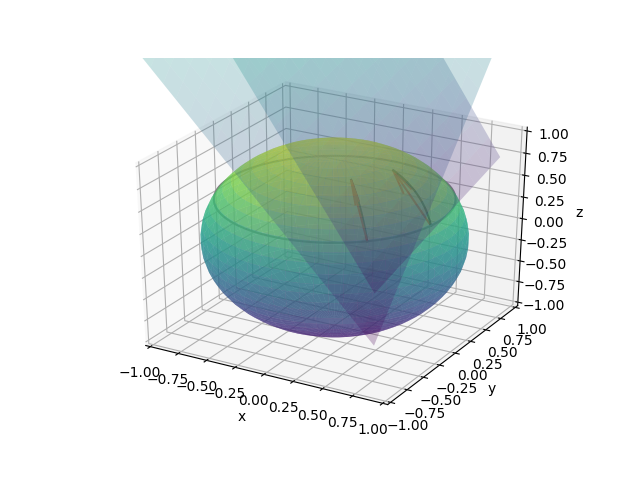
\includegraphics[width=0.8\linewidth]{1}
	\end{center}
	
	
	\vfill
	\newpage
	
	\section{Introducción}
	En esta práctica estudiaremos y haremos gráficas de la traslación paralela de un vector sobre una superficie (pseudo)-Riemanniana suave: en nuestro caso, una esfera unitaria en el espacio tridimensional, $s_1^2\subset\mathbb{R}^3$.
	
	Una \textbf{traslación o transporte paralelo} de una sección $X$ sobre una curva $\gamma$ de una variedad como $S_1^2$ cumple que la derivada direccional de $\gamma$ es 0. En este caso, un elemento de la fibra de esta variedad será un vector de un plano tangente sobre la esfera, y la curva escogida será un paralelo de la esfera. 
	
	\section{Material usado y metodología}
	
	En coordenadas polares, si $q(\phi,\theta)$ es un punto de la esfera con $\phi\in[0,2\pi)$ y $\theta\in[-\frac{\pi}{2},\frac{\pi}{2}]$, entonces la parametrización del paralelo $\theta_0$ es $\gamma_{\theta_0}(\phi) = q(\phi,\theta_0)$.
	
	El vector que vamos a transportar es $v_0=(0,\frac{\pi}{5})$ colocado en el punto $q\in(0,\theta_0)$, con $\theta_0$ variable.
	
	Las ecuaciones del transporte paralelo de un vector $v_0$ pueden obtenerse de la condición, mencionada anteriormente, de que la derivada direccional sobre la curva $\gamma$ es 0. 
	
	En función del ángulo $\phi$, se obtiene un sistema lineal de ecuaciones diferenciales cuya solución es $v$, de componentes $v^1$ y $v^2$:
	
	\[ v^1(\phi) = v_0^2 \frac{\sin(\phi\sin(\theta_0))}{\cos(\theta_0)} \]
	\[ v^2(\phi) = v_0^2 \cos(\phi\sin(\theta_0)) \]
	
	
	\subsection{Apartado \textit{i})}
	En el primer apartado, definimos una sucesión $f(t)$ en función de un parámetro temporal $t\in[0,1]$, tales que $f(0)=v_0$ y $f(1)$ es la traslación de $v_0$ alrededor del paralelo entero ($\phi= 2\pi$). Además, la sucesión depende de $t$ cuadráticamente.
	
	Calcularemos cada elemento de la familia mediante la función \texttt{transp}, y adquiriremos, además, los puntos de origen donde colocar cada vector mediante la función \texttt{familia\_param}, que llama a su vez a \texttt{transp}.
	
	\subsection{Apartado \textit{ii})}
	En el segundo apartado, escogeremos dos valores de $\theta_0$. Esto define dos paralelos distintos, que dibujaremos en una gráfica mediante la función \texttt{paralelo}. 
	
	También colocaremos en la gráfica la malla de puntos que representa la esfera, como ya hemos hecho en prácticas previas. Es decir, discretizamos los puntos de la esfera $\in [0,2\pi)\times [-\pi/2, \pi/2]$ en una malla de $60\times30$, y se realiza la siguiente transformación cartesiana:
	\[
	\begin{aligned}
	x &= \sin(u) \times \sin(v)\qquad
	y &= \sin(u) \times \cos(v)\qquad
	z &= \cos(u) \times (1)_{i=1}^{|v|}
	\end{aligned}
	\]
	
	Con estos elementos constantes en cada fotograma, realizaremos una animación de la familia paramétrica $f(t)$ con los dos $\theta_0$ escogidos, y el intervalo $t\in[0,1]$ se discretizará de manera equidistante en 40 subintervalos. Para hacer la gráfica de cada vector, se llama a la función \texttt{get\_bipunto}, y a la función, de la librería \textit{matplotlib}, \texttt{quiver}.
	
	\section{Resultados y conclusiones}
	
	\subsection{Apartado \textit{i})}
	
	Como ya se ha descrito anteriormente, la familia escogida es $f(t)=v_t$, donde $v_t : [0,2\pi] \to S_1^2$:	
	\[v_t\left(\begin{array}{cc}\phi\\\theta_0\end{array}\right) 
	= v^2_0 \left(\begin{array}{cc}
	\frac{\sin(\phi\sin(\theta_0)\cdot t^2)}{\cos(\theta_0)}\\
	\cos(\phi\sin(\theta_0)\cdot t^2)
	\end{array}\right)\]
	
	\subsection{Apartado \textit{ii})}
	Los dos valores de $\theta_0$ escogidos son: $\theta_0^A=0$ y $\theta_0^B=-0.2\pi$. 
	
	A continuación\footnote{Para ver este gráfico en movimiento, se recomienda abrir este PDF en Adobe Reader u Okular.}, y así como en los archivos adjuntos, se encuentra la animación de la sucesión de funciones paramétricas $f(t)$. El vector que recorre el paralelo $\theta_0^A$ es el rojo, y $\theta_0^B$ el azul. Como podemos observar, en el segundo caso el vector trasladado no se corresponde con el original.
	
	\begin{center}
		\animategraphics[method=ocg,width=0.5\paperwidth,loop,autoplay]{6}{img/2_}{1}{40}
	\end{center}
	
	Gracias a esta práctica hemos podido experimentar de primera mano cómo se define el transporte paralelo de vectores, que puede parecer trivial en el espacio $\mathbb{R}^n$, en otra variedad como es una esfera. Con ello hemos adquirido un mejor entendimiento de este objeto y de las curiosas propiedades que trae su curvatura.
	
	\newpage
	\section{Código}\label{codigo}
	
	\lstinputlisting[language=Python]{p8_rubiomadrigalcelia.py}
	
\end{document}
